\subsection{Durchführung des manuellen Netzwerk-Testplans vom 30.08.2015}

\textbf{Durchgeführt von:} Matthias Hofmann

\textbf{Änderungen vorgenommen in Commit:} keine Änderungen nötig

\paragraph{Teil N-i Allgemeine Informationen zu den Testergebnissen}

\paragraph{Test N-i.1 Packet Attribute im Dashboard}

Die Spaltenfunktionalität im Dashboard ist der Reihe nach aufgelistet:

\begin{itemize}
  \item Gerät, das die Informations ans Dashboard sendet
  \item Ereignis, das den Informationsautsch auslöst
  \item Uhrzeit des Ereignis
  \item Verwendetes Übertragungsprotokoll
  \item Adresse des Empfängers(Falls Ereignis = ``SEND'')
  \item Packetdetails
\end{itemize}

In der sechsten Spalte im Dashboard werden Details der Übertragung dargestellt. Dabei ist die eindeutige ID der Nachricht das zweite Attribut vom Packet. Desweiteren steht \glqq routing=1\grqq~ für Senden via Flooding und \glqq routing=2\grqq~ für Senden via DRS-Adaption.

\paragraph{Test N-i.2 Zeiten der Nachrichten im Dashboard}

Die angegebenen Zeiten der Ereignisse im Dashboard wirken auf den ersten Blick unwahrscheinlich. Zum Beispiel wird in Test II) 1 ein Acknowledgement zuerst empfangen, bevor es gesendet wurde. Dies liegt daran, dass die Übertragungn des Acknowledgements per Bluetooth stattgefunden hat und das Gerät, das diese empfangen hat, eine schnellere Verbindung zum Dashboard-Server hatte. Somit wurde das Dashboard zuerst über das Ankommen des ACK informiert und dann erst über das Versenden.

Ein weiterer Störfaktor ist, dass die gelisteten Zeiten von den Geräten selbst gemessen wurden. Da diese nicht synchronisiert wurden ensteht hier eine Ungenauigkeit. Diese ist allerdings vernachlässigbar, da für die hier durchgeführten Tests keine exakte Zeitbestimmung notwendig ist und durch logisches Nachdenken die korrekte Reihenfolge der Nachrichten bestimmt werden kann.


\paragraph{Teil N-ii Testfälle für die allgemeine Übertragung}

\paragraph{Test N-ii.1 Test der direkten Übertragung via Flooding / Bluetooth}

Der Test war erfolgreich.

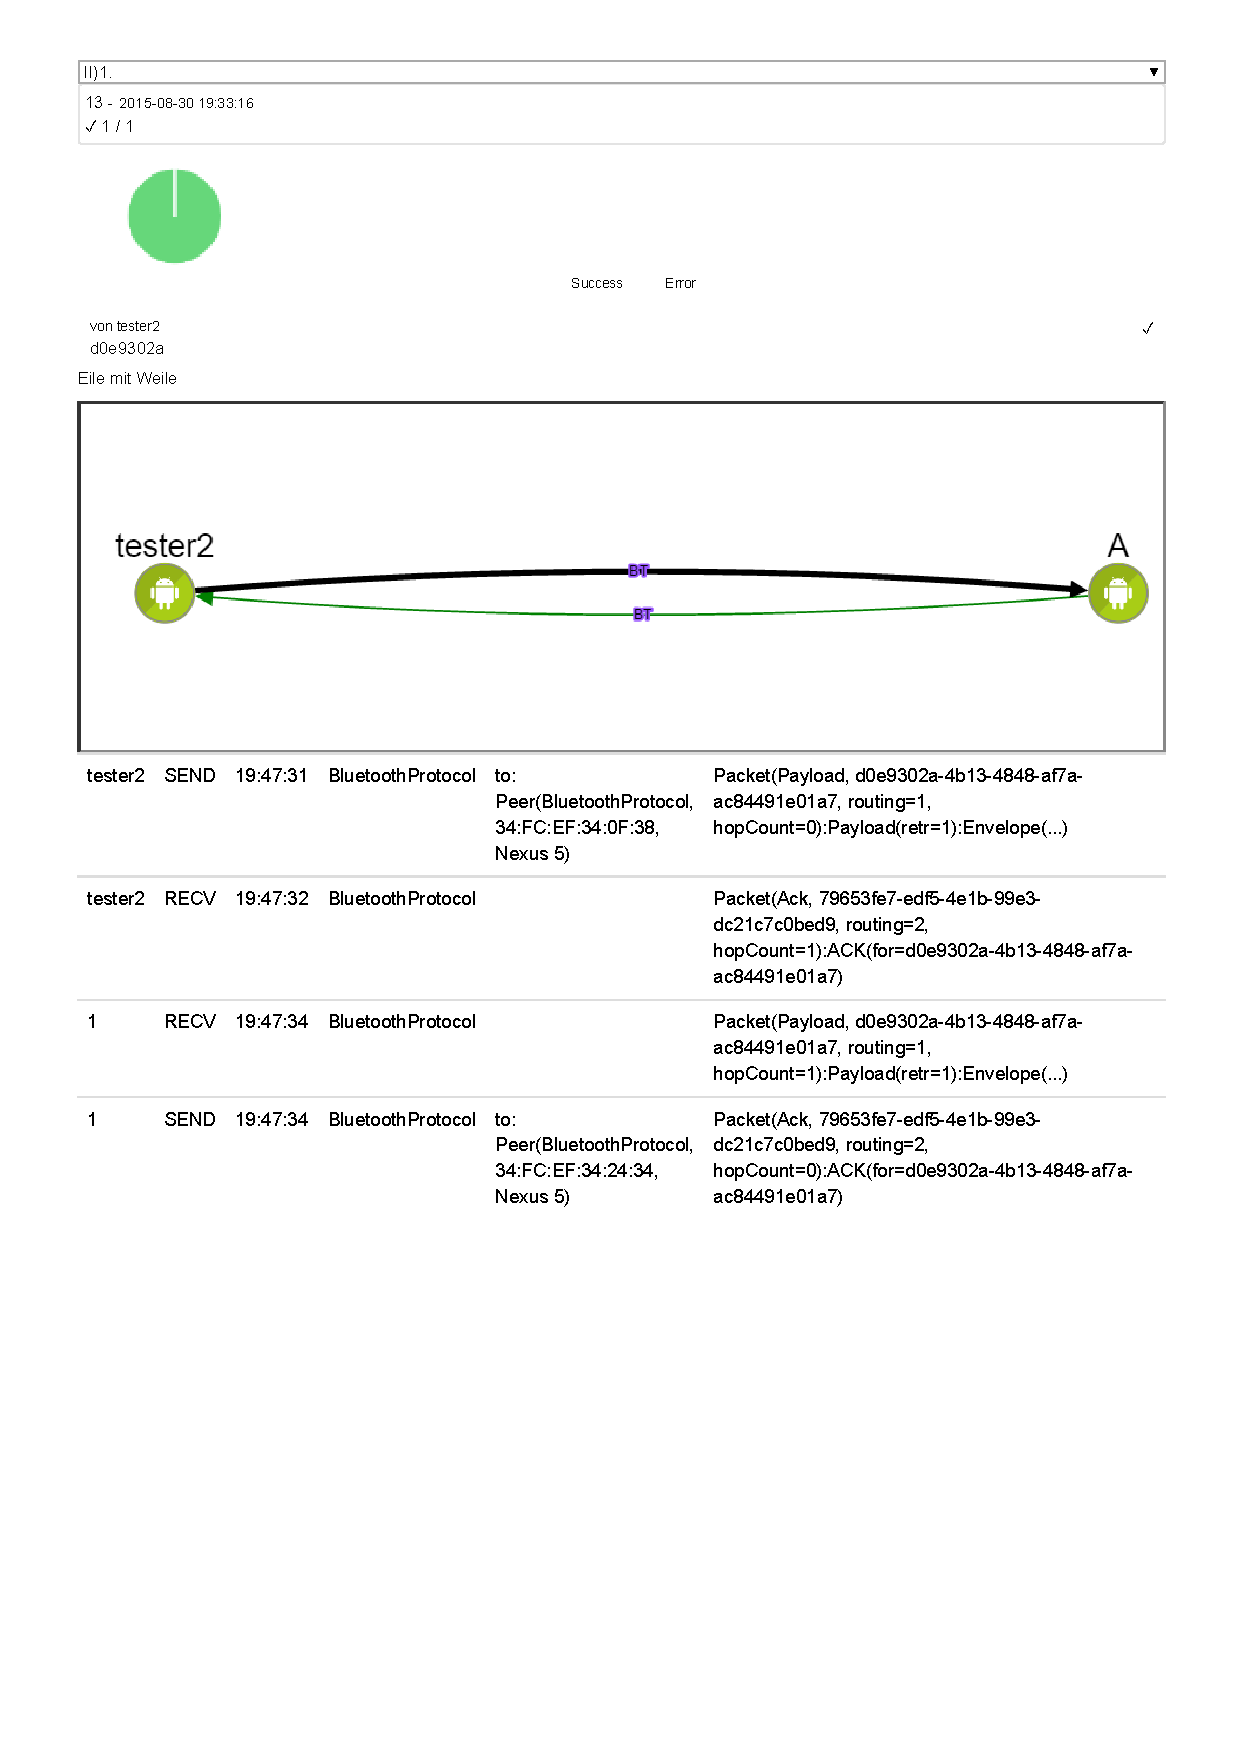
\includepdf[offset=-0.8cm 0,scale=.8,pagecommand={}]{belege/manuelle-tests/netzwerk/Dashboardauszuege/Netzwerktest_II-1.pdf}

\paragraph{Test N-ii.2 Test der direkten Übertragung via DSR / Bluetooth}

Der Test war erfolgreich.

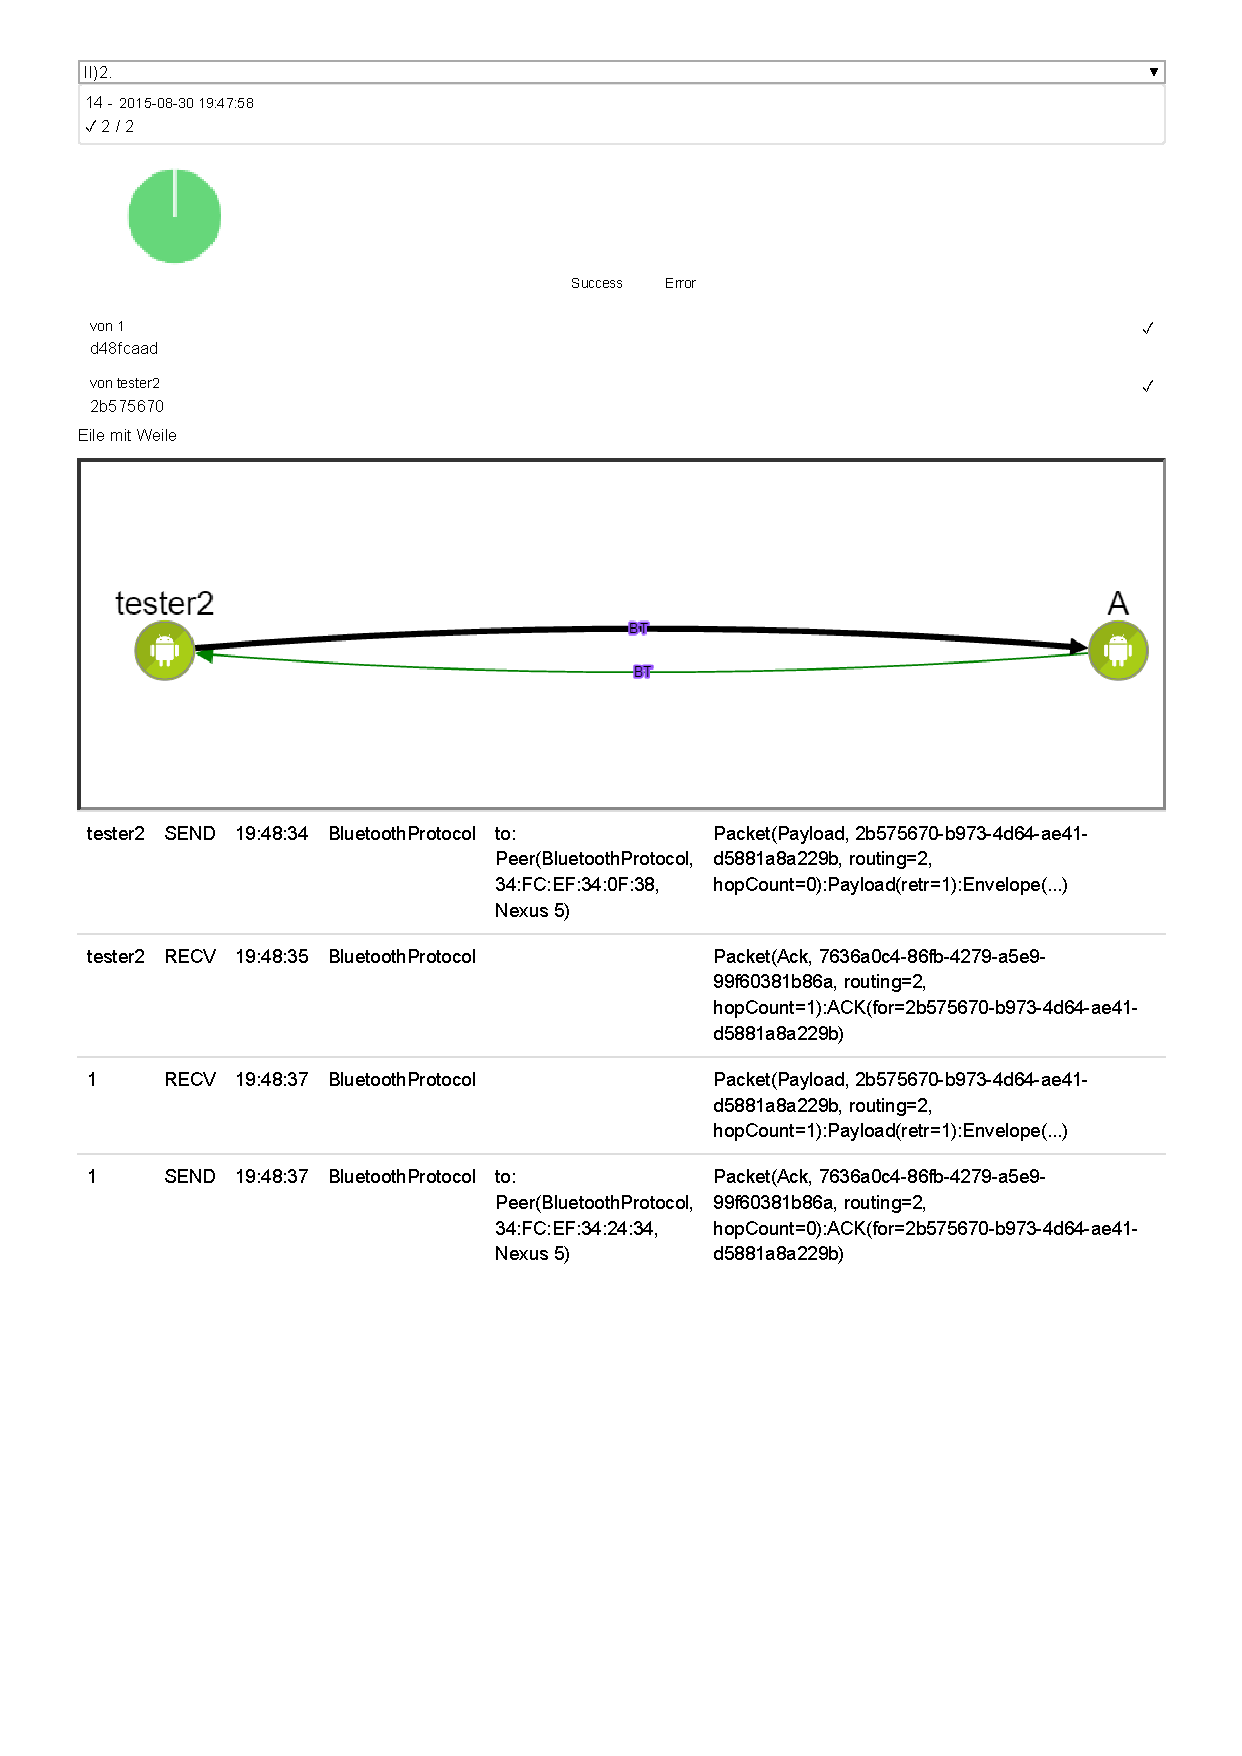
\includepdf[offset=-0.8cm 0,scale=.8,pagecommand={}]{belege/manuelle-tests/netzwerk/Dashboardauszuege/Netzwerktest_II-2a.pdf}
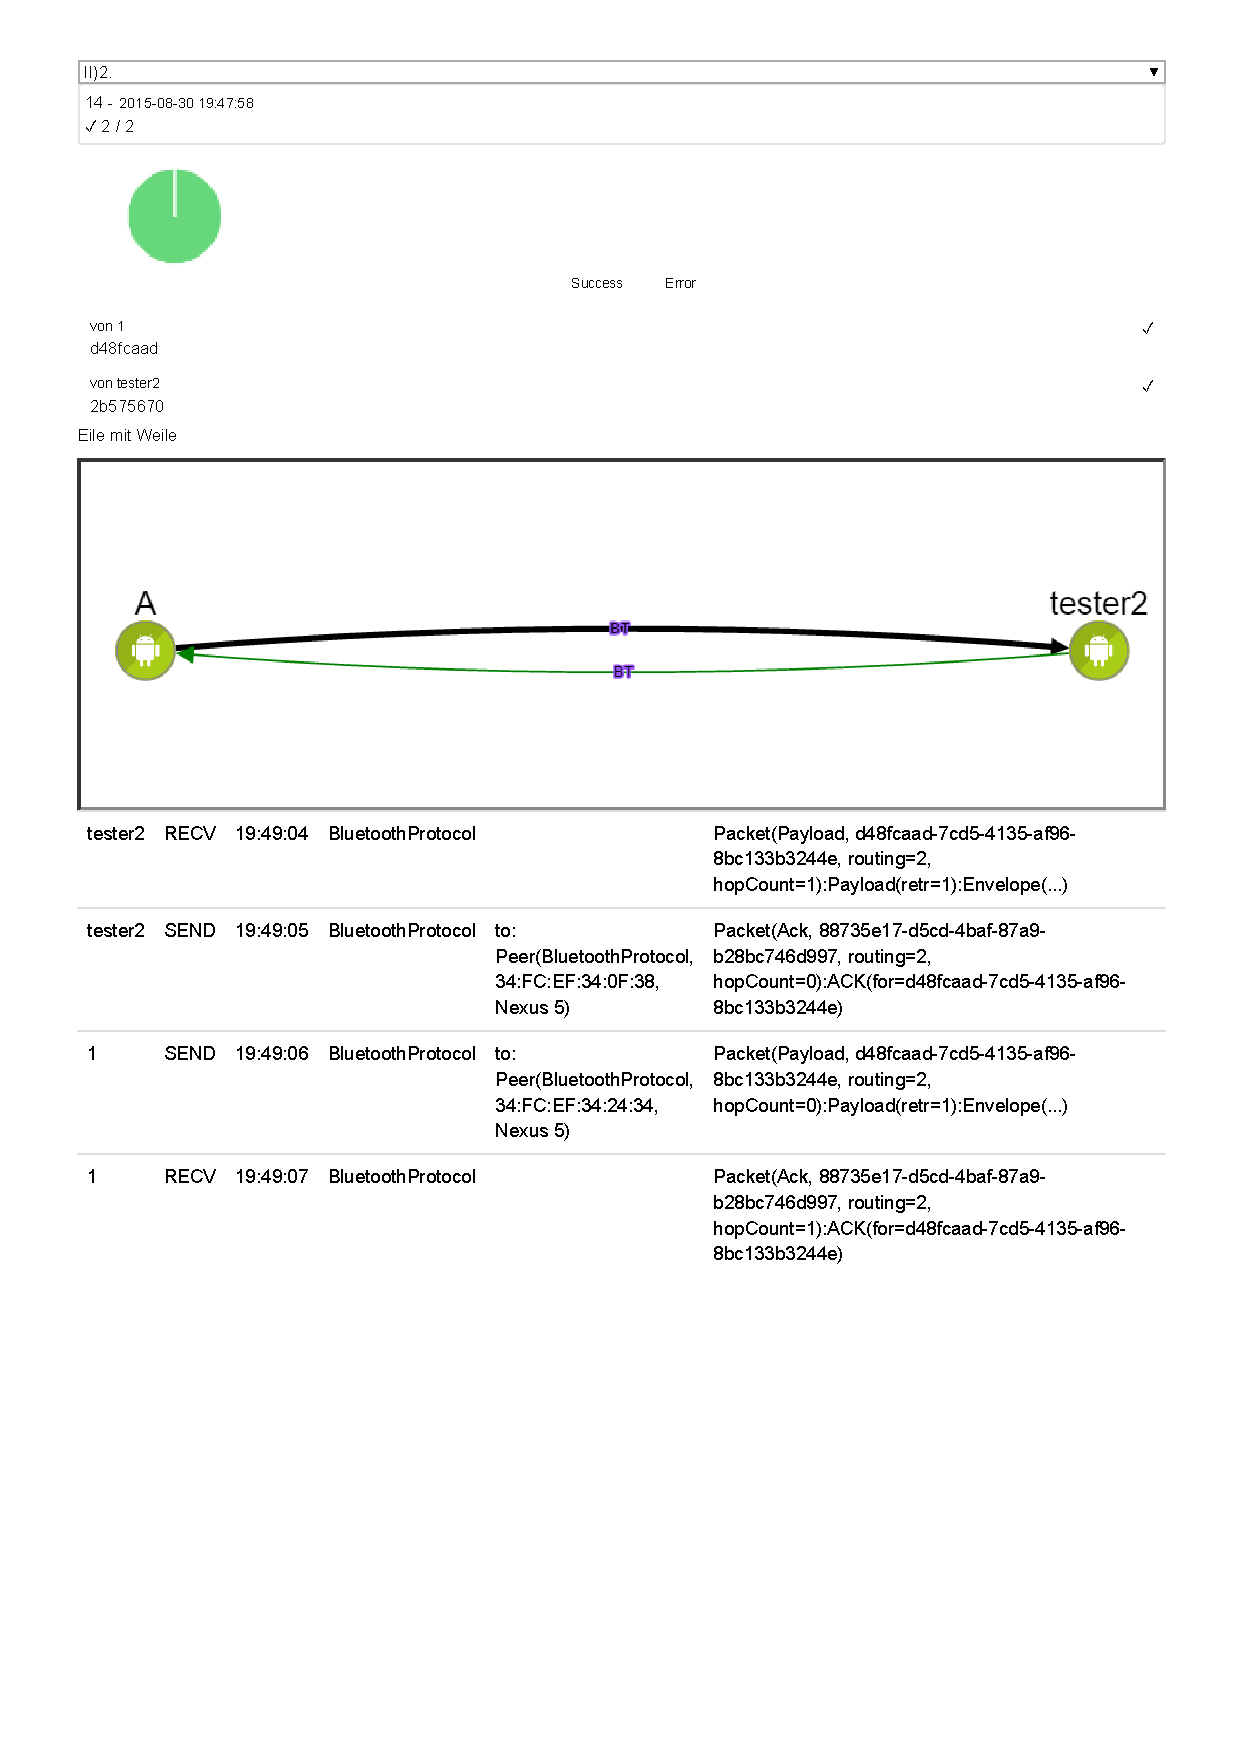
\includepdf[offset=-0.8cm 0,scale=.8,pagecommand={}]{belege/manuelle-tests/netzwerk/Dashboardauszuege/Netzwerktest_II-2b.pdf}

\paragraph{Test N-ii.3 Test der direkten Übertragung via Server / Google Cloud Messaging}

Der Test war erfolgreich.

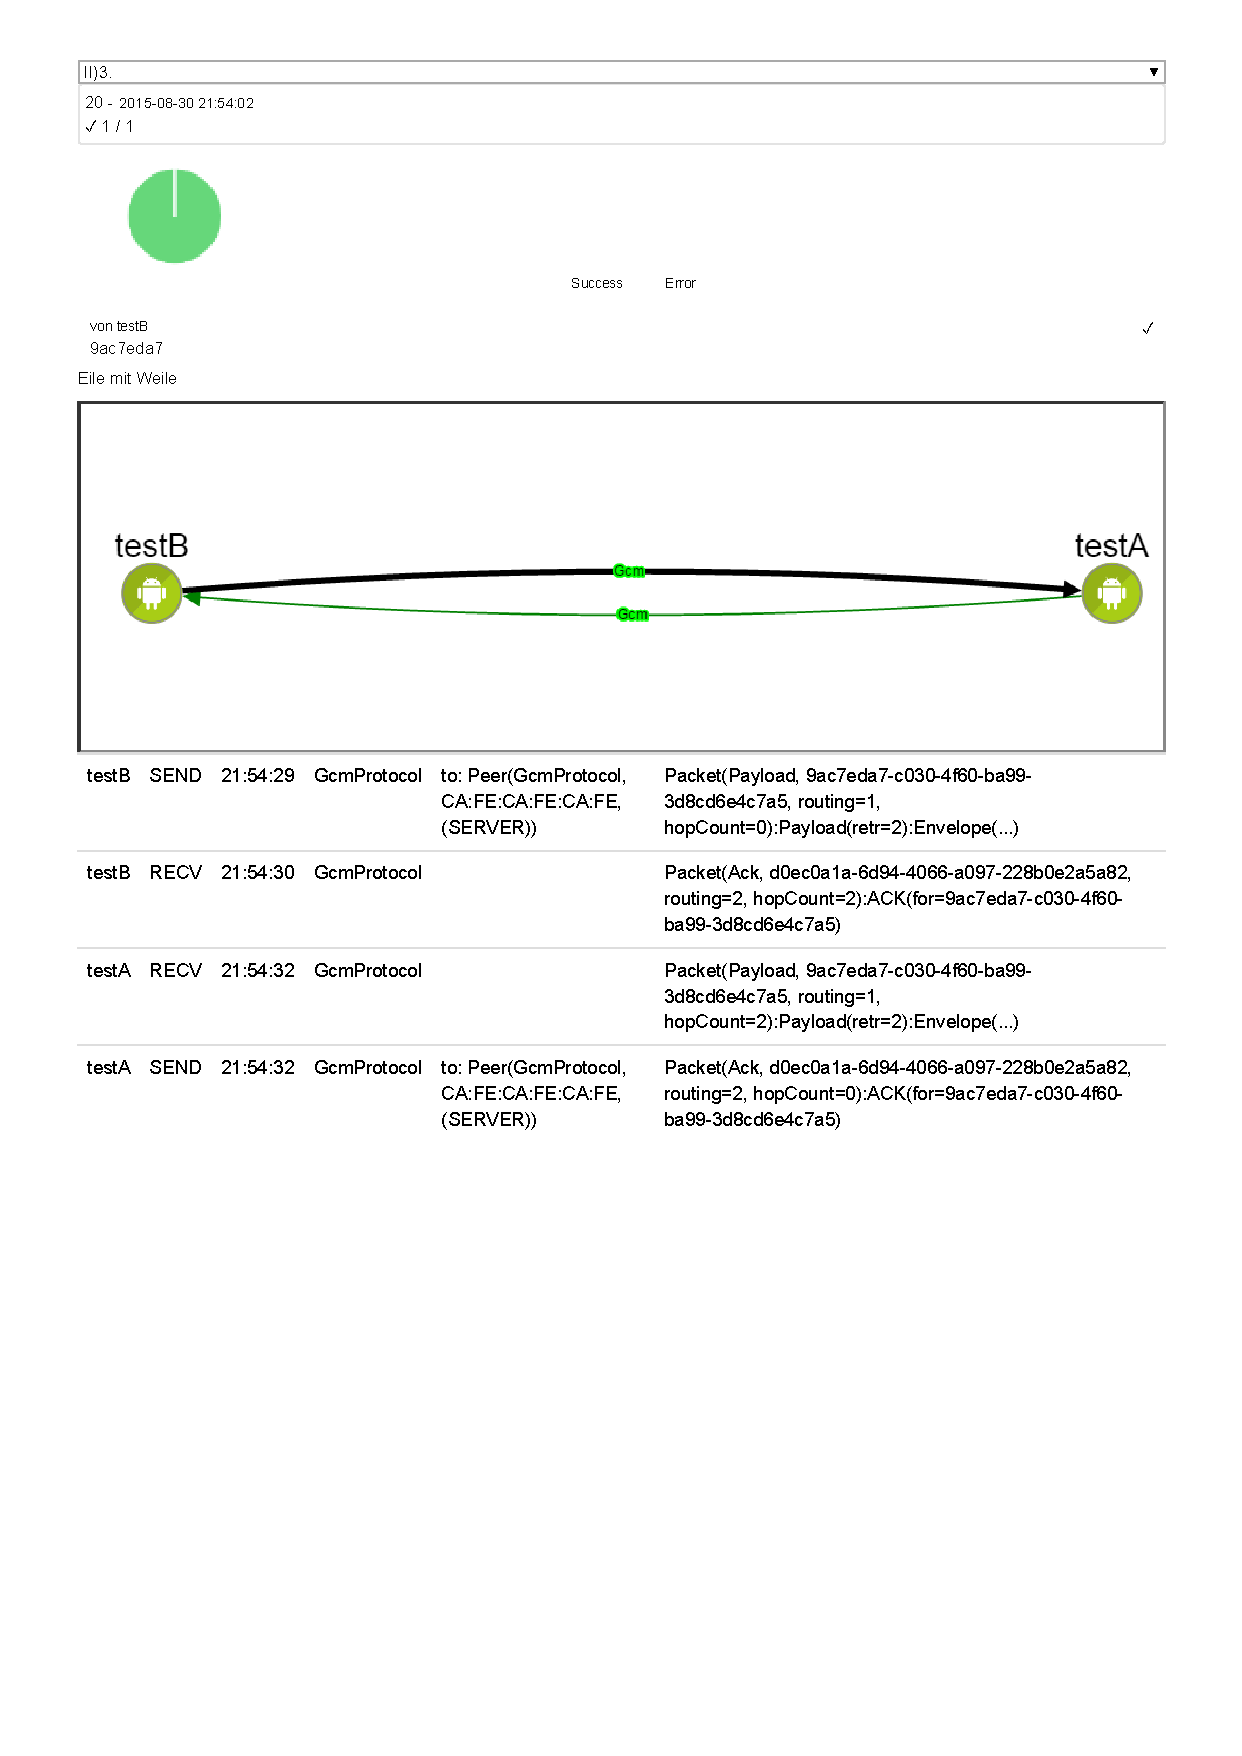
\includepdf[offset=-0.8cm 0,scale=.8,pagecommand={}]{belege/manuelle-tests/netzwerk/Dashboardauszuege/Netzwerktest_II-3.pdf}


\paragraph{Teil N-iii Testfälle für Wegfindung per Flooding und einfaches Routing}

\paragraph{Test N-iii.1 Bluetooth-Wegfindung - Flooding mit drei Knoten}

Der Test war erfolgreich.

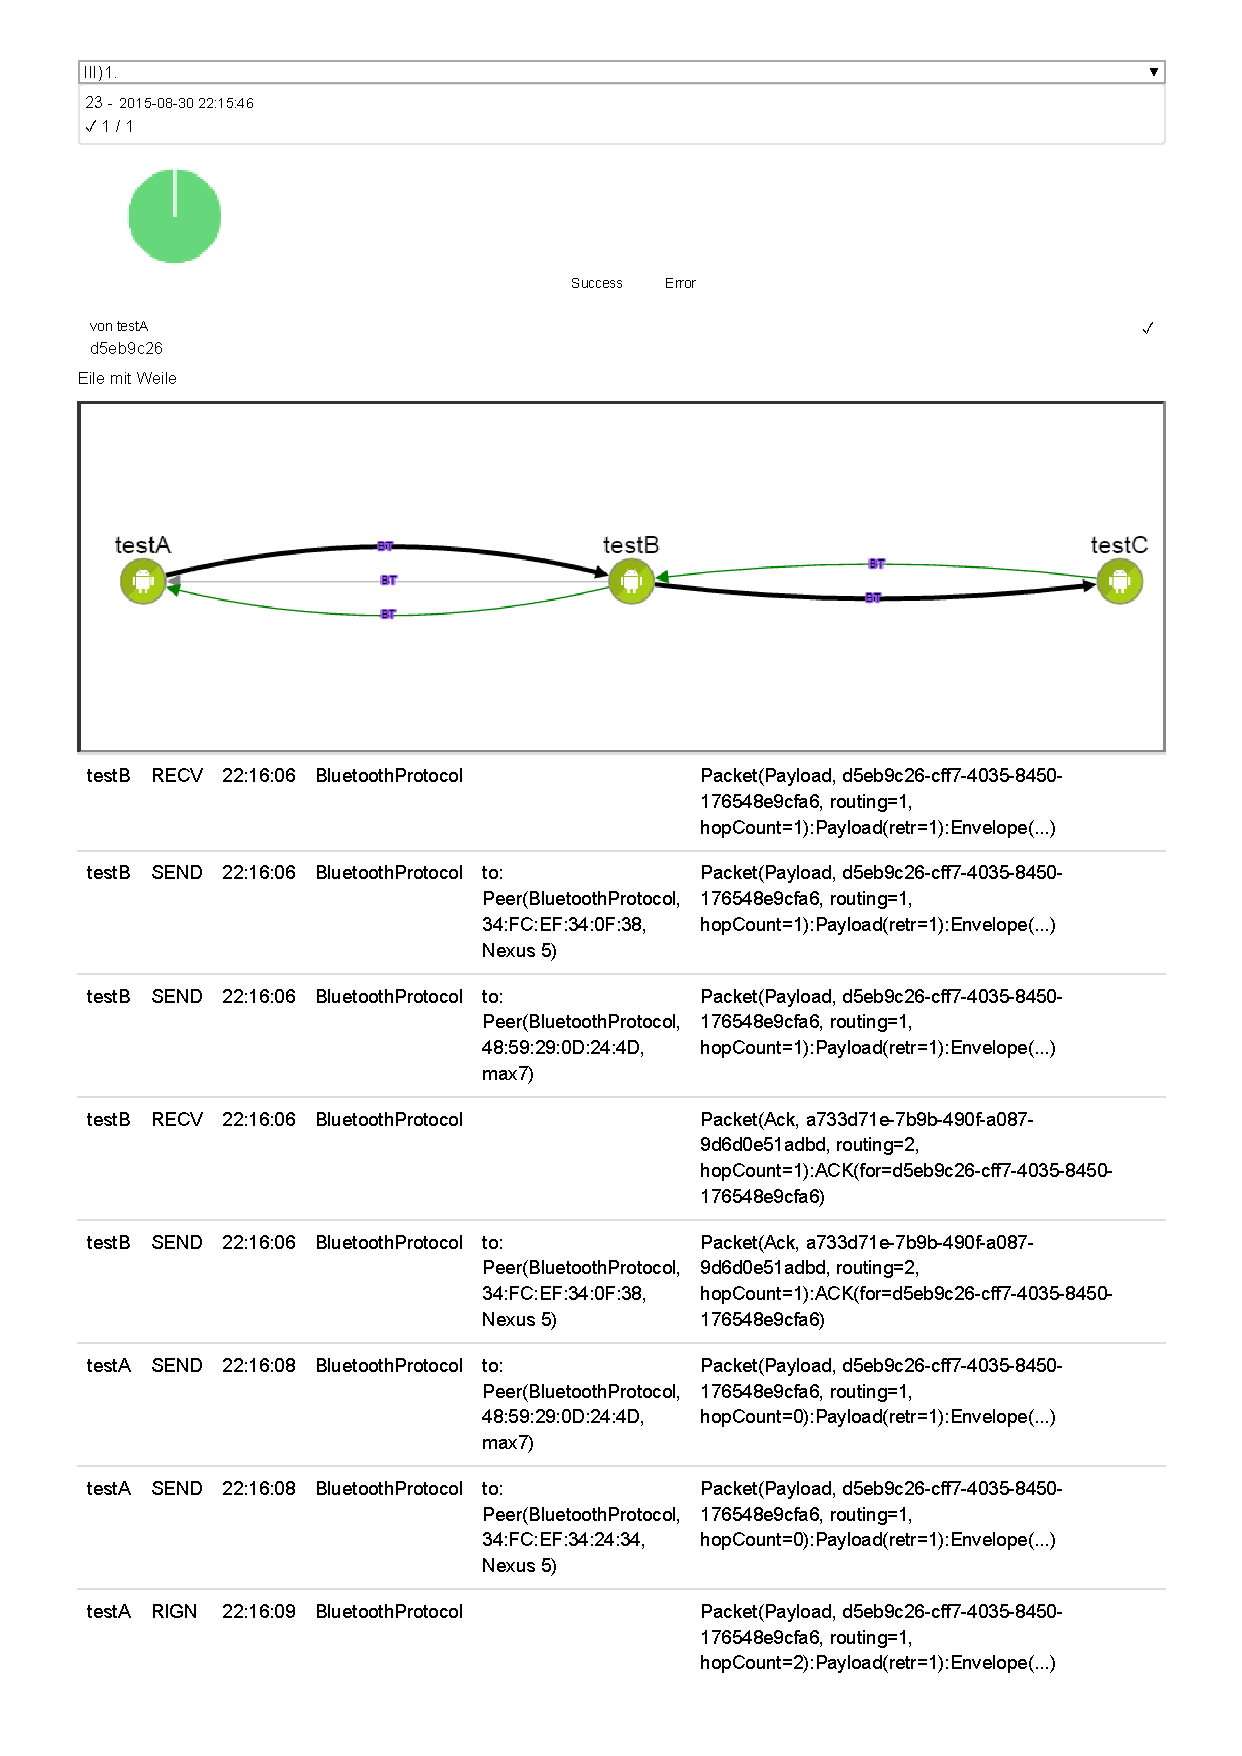
\includepdf[offset=-0.8cm 0,scale=.8,pagecommand={}]{belege/manuelle-tests/netzwerk/Dashboardauszuege/Netzwerktest_III-1.pdf}

\paragraph{Test N-iii-2 Bluetooth-Wegfindung zum nächsten Knoten mit Internetverbindung}

Der Test war erfolgreich.

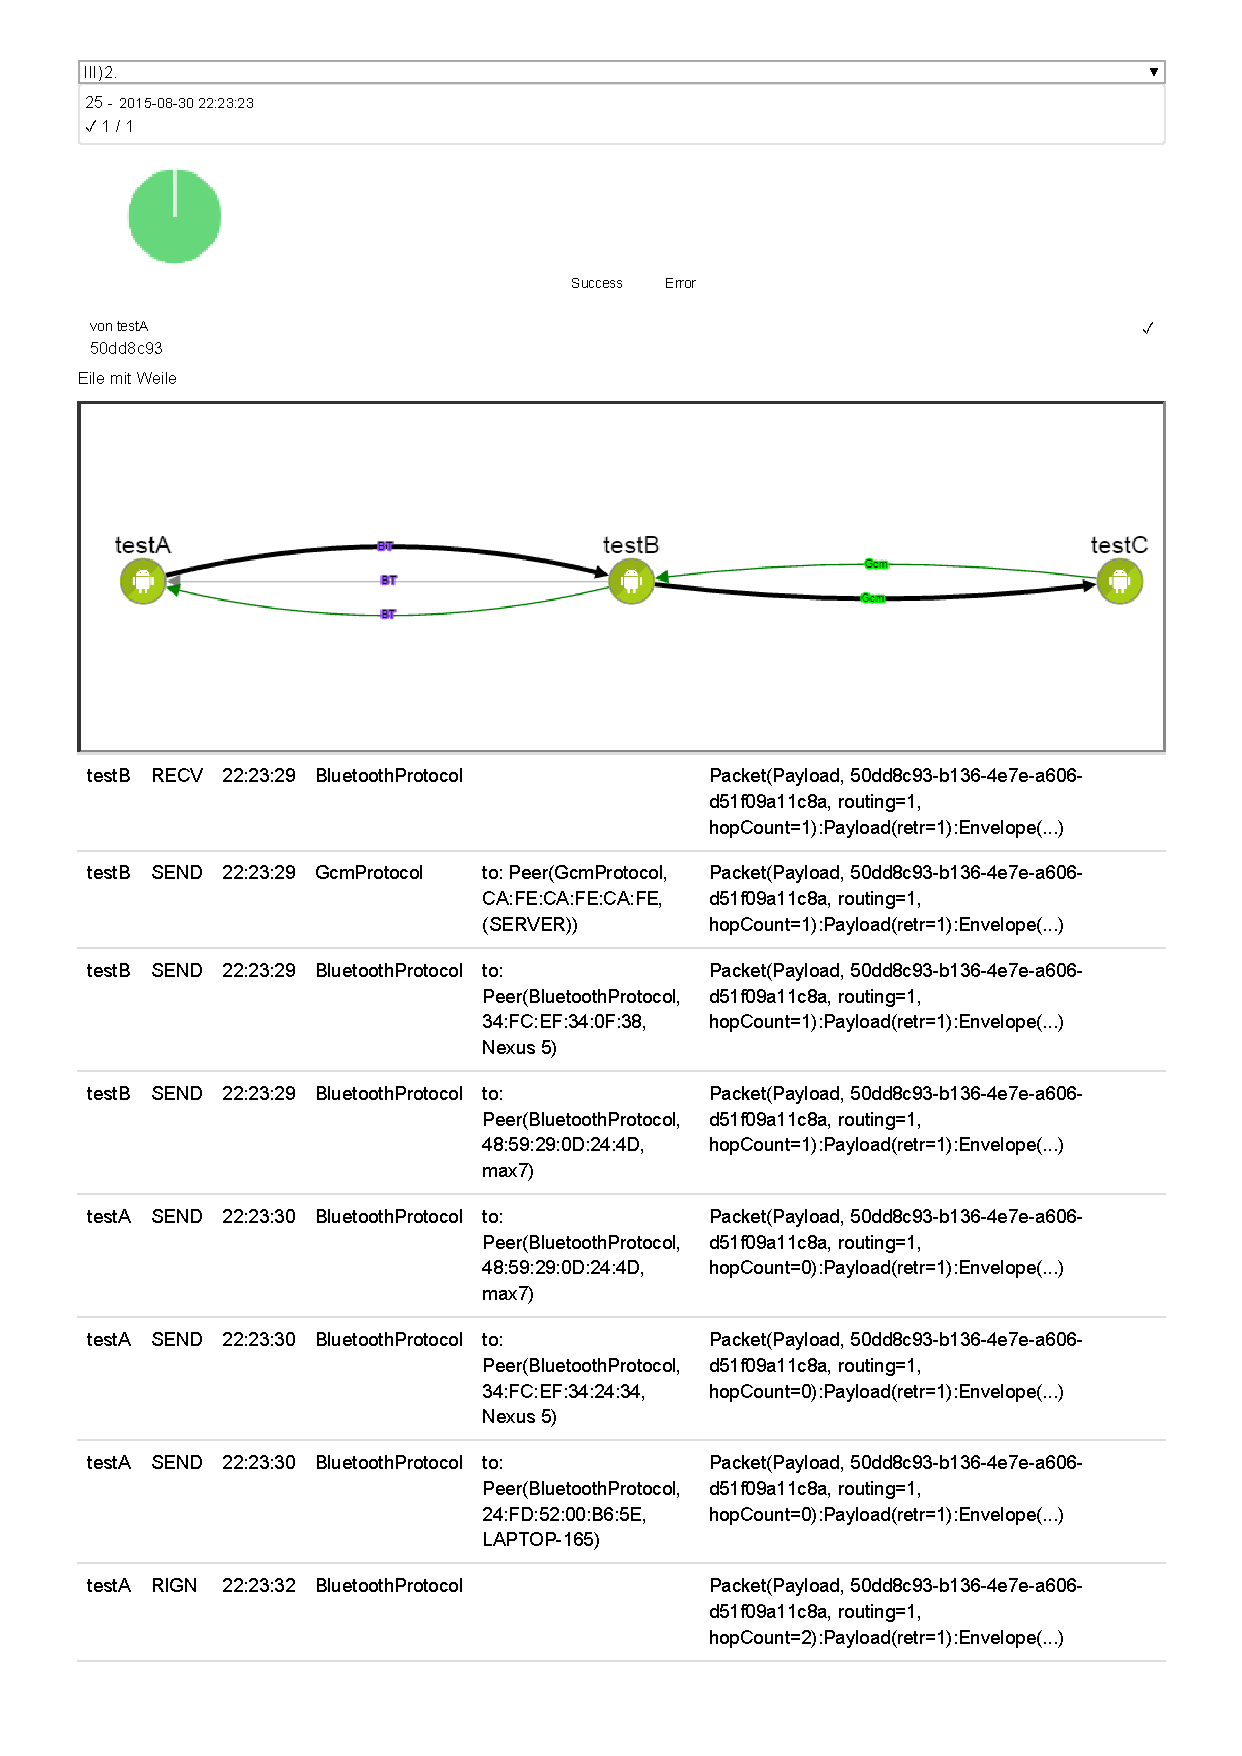
\includepdf[offset=-0.8cm 0,scale=.8,pagecommand={}]{belege/manuelle-tests/netzwerk/Dashboardauszuege/Netzwerktest_III-2.pdf}


\paragraph{Teil N-iv Testfälle für sich verändernde Routen}

\paragraph{Test N-iv.1 \glqq Abreißende\grqq~ Bluetooth-Verbindung}

Der Test war erfolgreich.

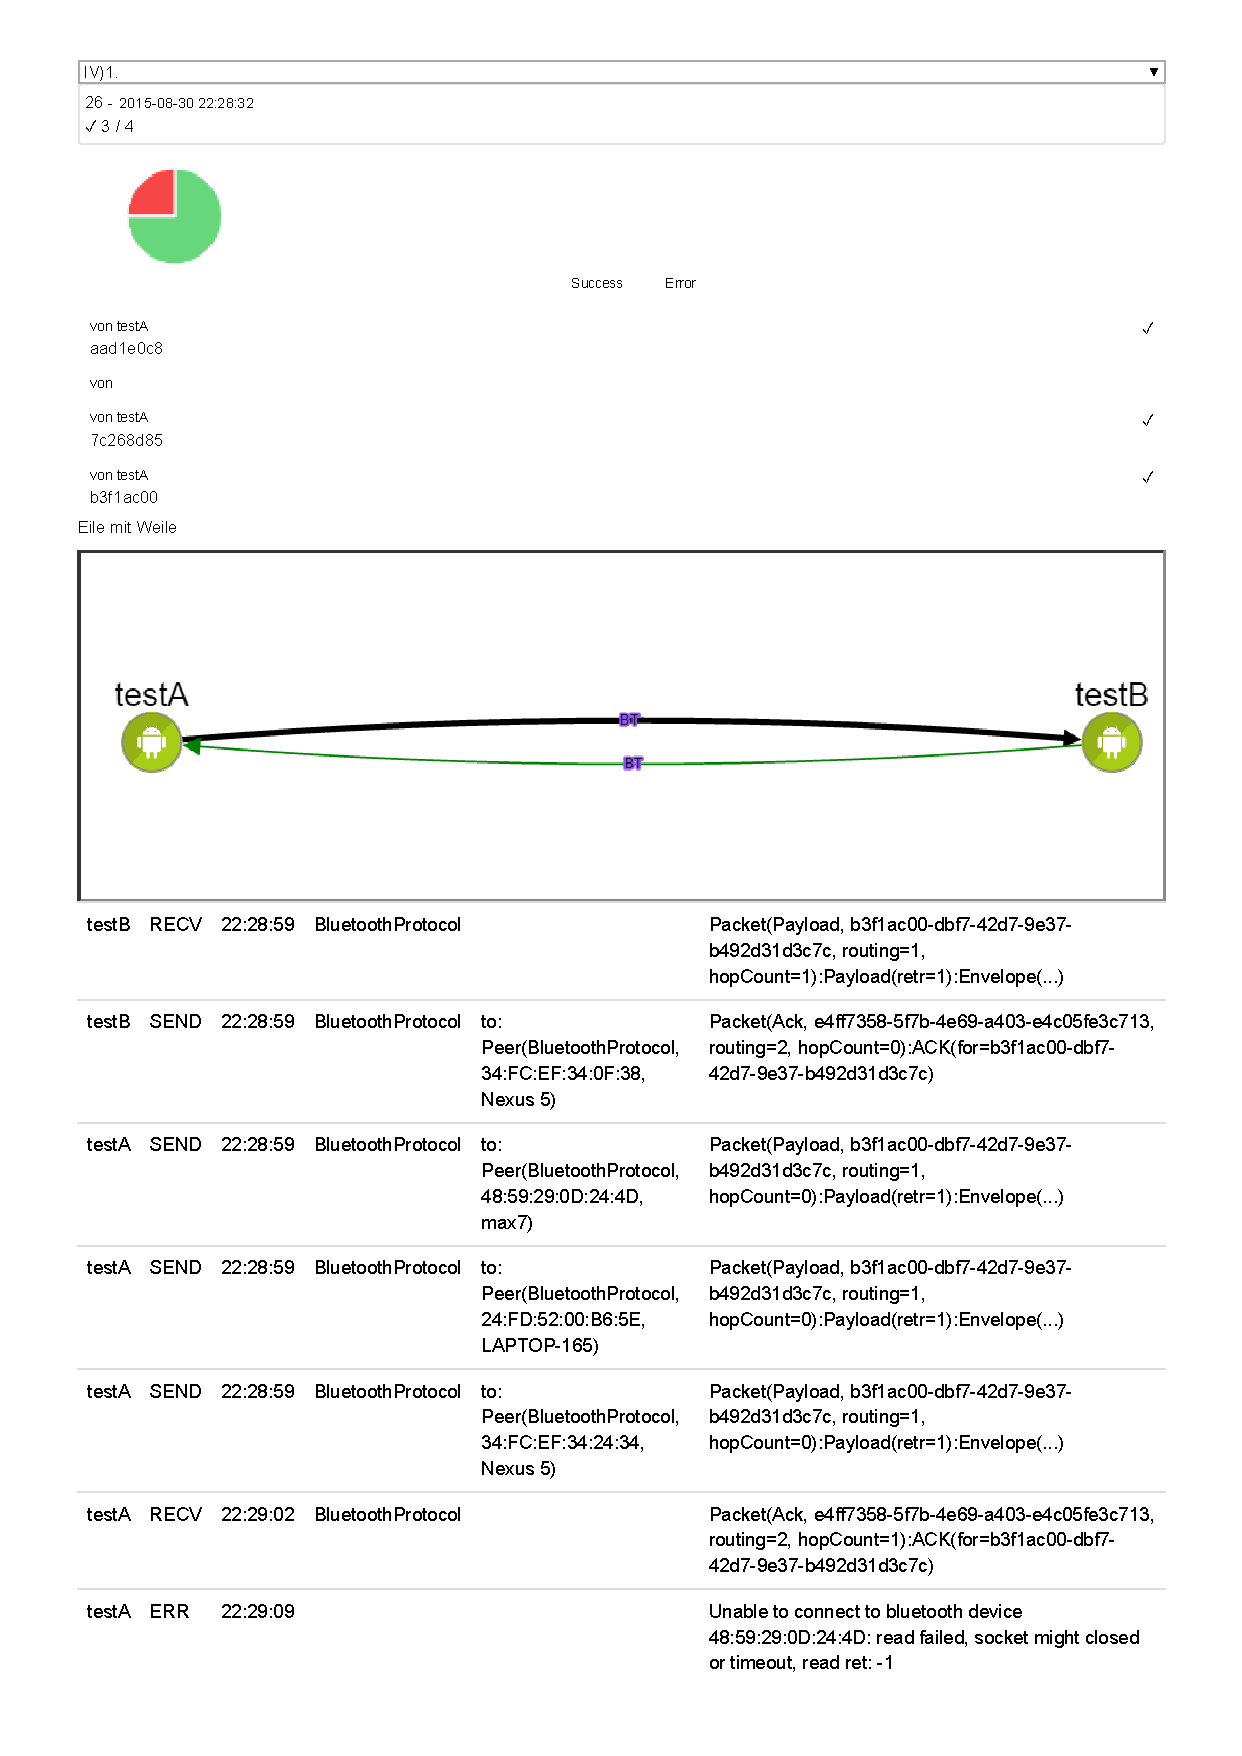
\includepdf[offset=-0.8cm 0,scale=.8,pagecommand={}]{belege/manuelle-tests/netzwerk/Dashboardauszuege/Netzwerktest_IV-1a.pdf}
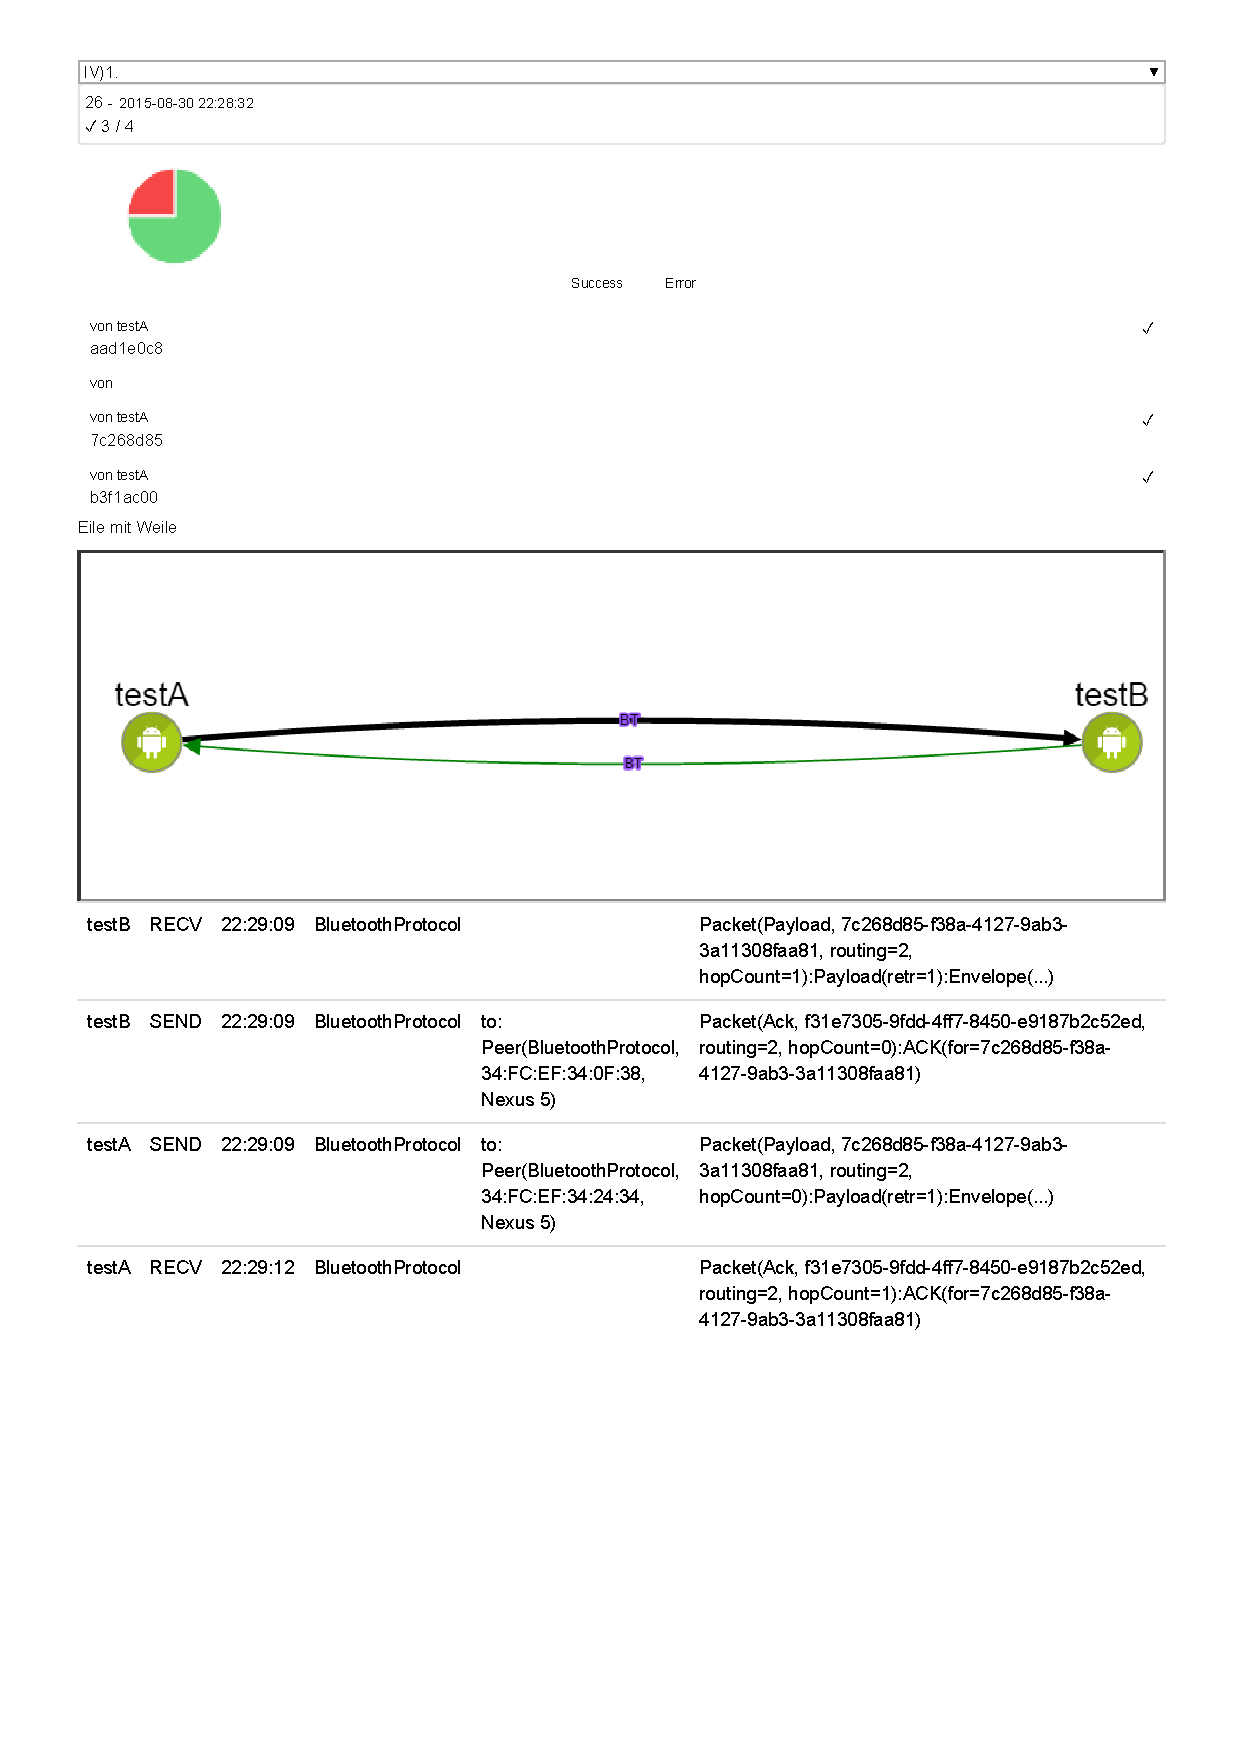
\includepdf[offset=-0.8cm 0,scale=.8,pagecommand={}]{belege/manuelle-tests/netzwerk/Dashboardauszuege/Netzwerktest_IV-1b.pdf}
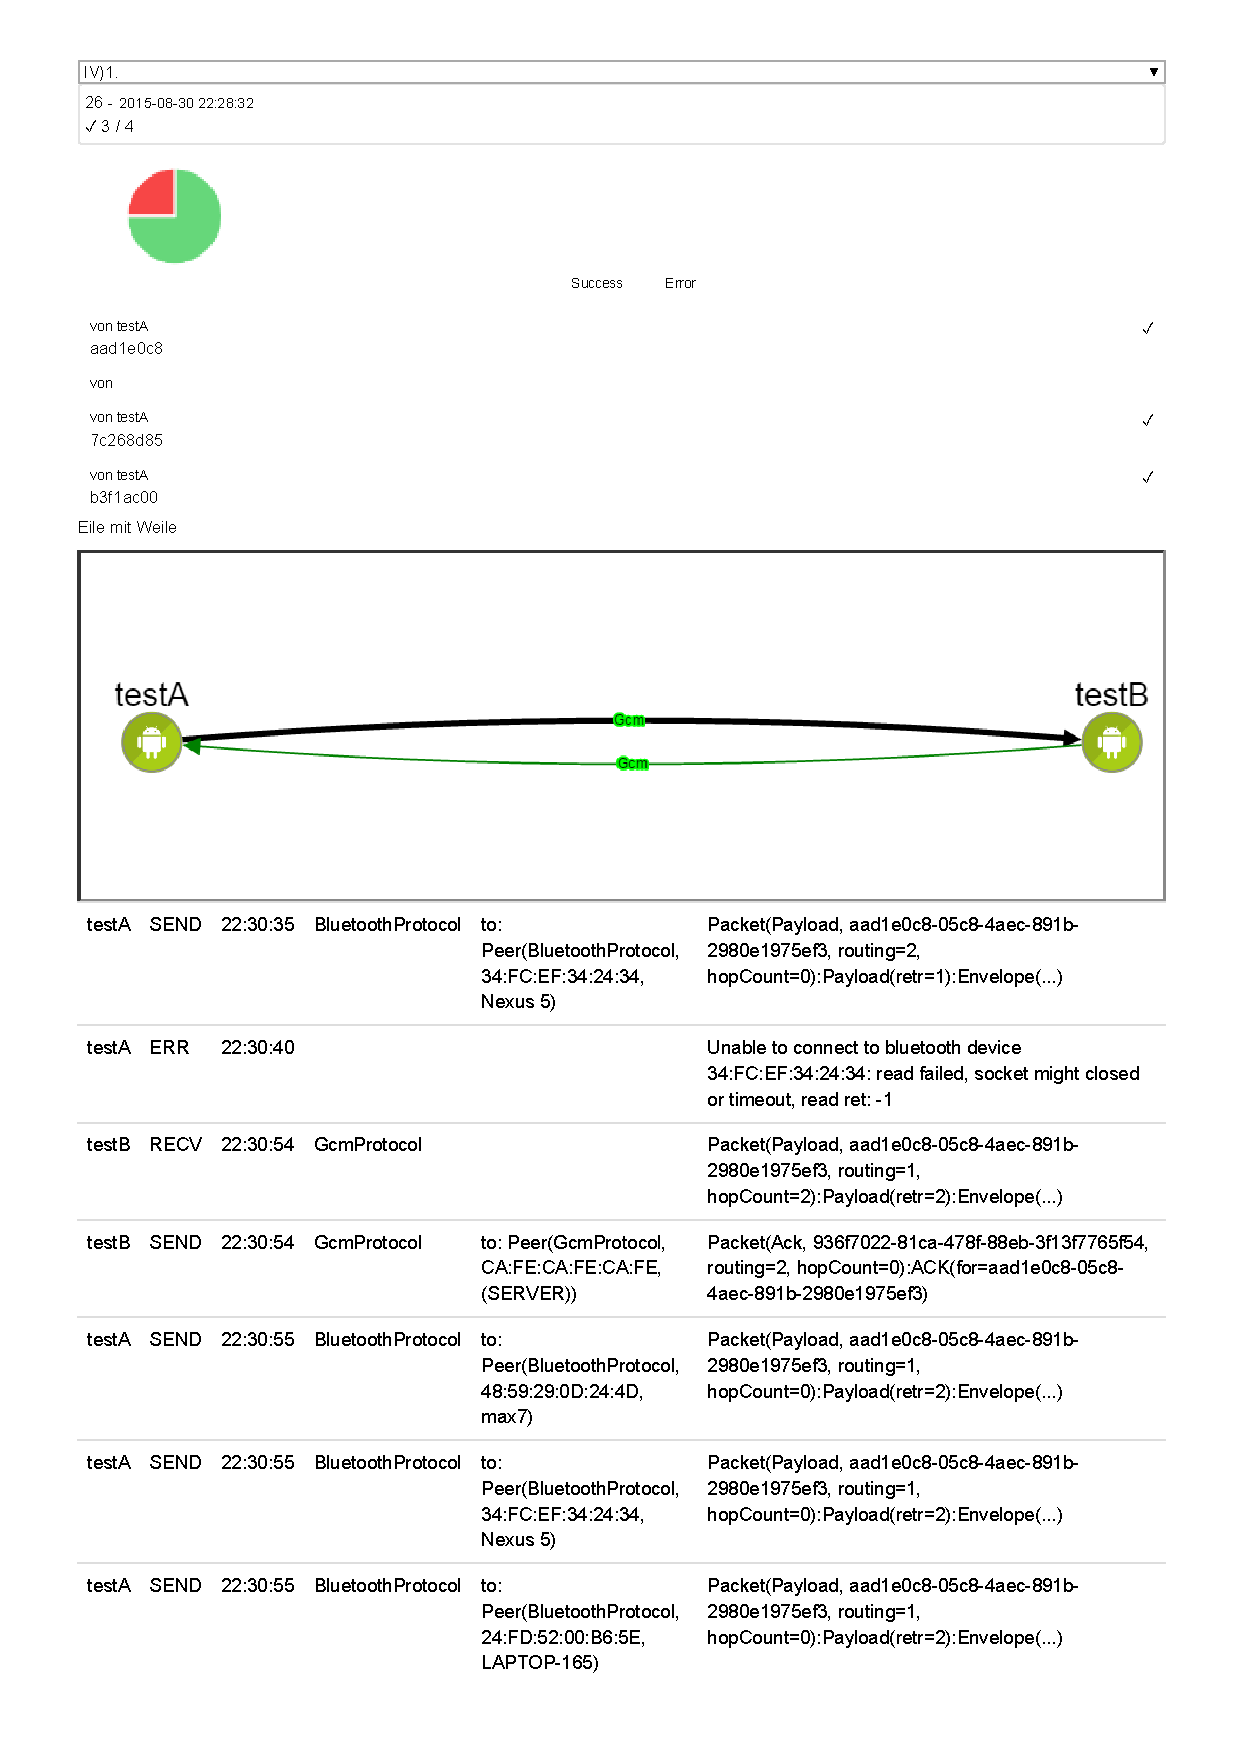
\includepdf[offset=-0.8cm 0,scale=.8,pagecommand={}]{belege/manuelle-tests/netzwerk/Dashboardauszuege/Netzwerktest_IV-1c.pdf}
